\chapter{Trabalhos Correlatos}

Neste capítulo serão analisados alguns projetos que focam no rastreamento, identificação e localização de pessoas em um ambiente inteligente. 

Alguns dos projetos estudados utilizam técnicas de identificação e rastreamento multimodais. Estas são compostas por informações redundantes providas por alguns tipos diferentes de sensores como, por exemplo, sensores de áudio e vídeo que fornecem dados audiovisual  das pessoas no ambiente .

Mesmo assim, somente as técnicas de identificação, localização e rastreamento monomodais que utilizarem imagens (cor, intensidade ou profundidade) como entrada serão descritas e analisadas.

Dentre os projetos estudados, destacam-se os seguintes projetos....(falar o pq).

\section{Projeto CHIL}

O Projeto CHIL (\textit{Computers in the Human Interaction Loop})~\cite{chil, computerschil} é composto por uma equipe de quinze laboratórios internacionais de pesquisa acadêmica e industrial.

Eles colaboram entre si no desenvolvimento de serviços que visam ajudar as pessoas de forma proativa durante suas atividades diárias. Em especial, possui foco em interações entre grupo de pessoas como, por exemplo, serviços que facilitam a colaboração em reuniões e em salas de palestras. 

Dentre os protótipos que foram desenvolvidos no projeto destacam-se um ambiente de trabalho perceptivo e colaborativo e um sistema perceptivo de assistência a um escritório virtual.

O Projeto CHIL utiliza uma combinação de algoritmos monomodais para criar um sistema de rastreamento e identificação multimodal utilizando dados audiovisual das pessoas no ambiente. Do ponto de vista do áudio, é importante mencionar que o Projeto CHIL representa uma das primeiras tentativas de realizar e avaliar sistematicamente rastreamento acústico com uma rede distribuída de microfones. Porém, será focado os algoritmos que utilizam somente dados visuais para realizar tais tarefas.

Referente a localização das pessoas no ambiente, o projeto focou somente na localização das pessoas que ``falam''~\cite{speaker-localization}.

Como a equipe deste projeto é composta por vários laboratórios, diferentes sistemas de rastreamento e identificação foram desenvolvidos. Contudo, será relatado somente aqueles que se destacaram.

\subsection{Rastreamento de Pessoas}

A pesquisa sobre rastreamento de pessoas foi focada principalmente no rastreamento de pessoas dentro de um ambiente inteligente. O rastreamento tinha o objetivo de determinar,  de maneira contínua, as coordenadas dos ocupantes na imagem.

Os sensores utilizados no ambiente inteligente do Projeto CHIL incluem:	
	\begin{itemize}
		\item um mínimo de quatro câmeras fixas instaladas nos cantos do ambiente, com campos de visão sobrepostos;
		\item uma câmera com grande ângulo de visão fixa com vista para o ambiente inteiro;
		\item três arrays de microfones em forma de T de 4 canais cada;
		\item um microfone de Mark III de 64 canais;
	\end{itemize}

Era esperado que essa grande quantidade de sensores disponíveis pudesse ser vista como uma vantagem, por oferecerem uma grande redundância nas informações capturadas e proveria uma boa ``cobertura'' do ambiente superando problemas como oclusão. Porém, foi observado no projeto que essa redundância se tornou um grande desafio, pois surgem problemas como sincronização dos dados, transferência de processamento distribuído, fusão de espaço-temporal, entre outros.

Durante o projeto, muito progresso foi feito. No início, os sistemas eram de uma única modalidade com inicialização manual, utilizando recursos simples e acompanhamento de no máximo uma pessoa. Estes sistemas evoluíram para um sistema totalmente automático, com auto-inicialização, em tempo real, utilizando uma combinação de recursos capaz de rastrear alvos múltiplos.

Sobre os algoritmos de rastreamento visual, duas abordagens principais foram seguidas pelos vários sistemas de rastreamento desenvolvidos no Projeto CHIL:

	\begin{enumerate}
		\item uma abordagem baseada em modelos, em que um modelo 3D do objeto rastreado é mantido renderizando-o nos pontos de vista da camêra.~\cite{chilref1,chilref2,chilref3}.
		\item  uma abordagem orientada a dados, onde sistemas de rastreamento 2D operam de forma independente sobre os diferentes ângulos de visão das câmeras e os dados do rastreamento pertencentes a um mesmo alvo são coletados no formato de um rastreamento 3D~\cite{chilref4,chilref5}.
	\end{enumerate}	

 Em termos de desempenho, foi observado no projeto que a abordagem baseada em modelos (1) geralmente prevê uma melhor acurácia, mas menos precisão do que a abordagem orientada a dados (2).  O tratamento das oclusões e da associação dos dados dos sistemas de rastreamentos independentes são as desvantagens do modelo orientado a dados. Foi identificado,  nesse projeto, que rastrear rosto em vez de corpos inteiros diminui o impacto desses problemas.

 Foi observado que a abordagem baseada em modelo também torna mais fácil incorporar diversos tipos de recursos, como segmentos de primeiro plano, histogramas de cor, etc, aumentando a robustez do rastreamento. Porém, as dificuldades encontradas nesta abordagem se resume na inicialização automática e na atualização dos modelos das pessoas.

 Os testes dos sistemas de rastreamentos desenvolvidos foram feitos utilizando-se os dados dos seminários do prórpio Projeto CHIL.

% As abordagens de rastreamento por meio de áudio e vídeo foram combinas em um rastreamento multimodal. Esse rastreamento multimodal é, notavelmente, baseado em filtro de partículas uma vez que permitem uma integração flexível de recursos através dos sensores~\cite{chil}.

% No rastreamento multimodal, era esperado que a fusão dos diferentes tipos de dados proveria resultados mais precisos, eliminando, assim, os efeitos de decisões erradas tomadas por algum rastreamento monomodal. Porém, não aconteceu o que se esperava. O rastreamento multimodal é altamente dependente das tarefas e dados em mãos, e exige um cuidadoso equilíbrio na disponibilidade e qualidade dos dados~\cite{chil}.

\subsection{Identificação das Pessoas}


A fim de realizar identificação de forma natural e implícita, os sensores distribuídos no ambiente devem monitorar continuamente o espaço. Então, o sistema de identificação de pessoas em um ambiente inteligente deve operar em segundo plano, sem necessitar de atenção e cooperação dos usuários. 

A face foi escolhida por ser uma característica biométrica que permite uma identificação de forma natural e implícita~\ref{sec:biometria}. Com isso, a equipe do Projeto CHIL desenvolveu diferentes sistemas de reconhecimento facial utilizando diferentes algoritmos. 

Na tentativa de realizar o reconhecimento facial das pessoas presentes no ambiente inteligente, vários desafios foram encontrados no Projeto CHIL, como: grande variação da iluminação, sensores com baixa resolução, oclusão visual e dependendo da localização de uma pessoa e sua distância dos sensores, os dados recebidos podem variar.  Além do mais, foi observado que o fato das pessoas possuírem diferentes expressões faciais, cortes de cabelo, maquiagens, entre outros, dificultava ainda mais a tarefa. Mesmo assim, foi notado que o reconhecimento facial podia ser realizado de forma robusta utilizando múltiplos sensores no ambiente.

Como dados, o sistema do Projeto CHIL utiliza sequências de imagens fornecidas pelas várias câmeras no ambiente inteligente. A cada $\displaysyle 200ms$ imagens das caixas delimitadoras das faces (uma maneira de apontar a localização da face na imagem por meio de um enquadramento) e posições dos centros dos olhos são extraídas, como exemplificado na Figura~\ref{chil}, em que no canto inferior direito, pode-se observar a imagem da face extraída. 

As faces, então, são alinhadas utilizando os centros dos olhos ou as caixas delimitadoras das faces. Para obter robustez contra alguns erros, o sistema gera algumas imagens adicionais alinhadas modificando rótulos do centro dos olhos ou os rótulos das caixas delimitadoras das faces.

	\begin{figure}[hbt]
		\begin{center}
			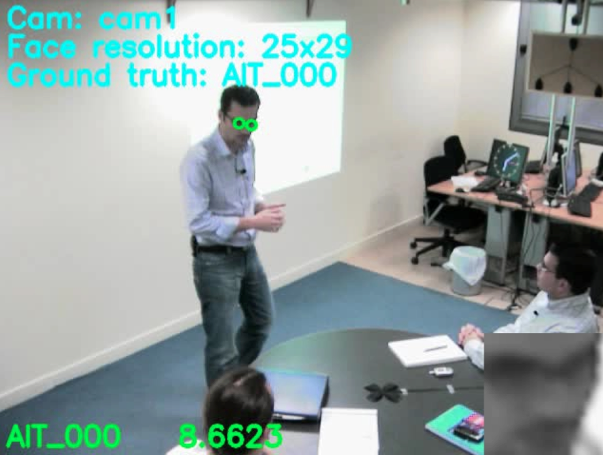
\includegraphics[scale=0.4]{figuras/3.TrabalhosCorrelatos/chil.png}
		\end{center}
		\caption{Exemplo do sistema de identificação facial do Projeto CHIL~\cite{chil}.}
		\label{chil}
	\end{figure}


O Projeto CHIL testou diferentes abordagens para reconhecimento facial. Uma delas realiza reconhecimento baseado em aparência utilizando transformada discreta de cosseno (DCT - \textit{Discrete Cosine Transform})~\cite{chilref6, chilref7}. Abordagens baseadas em PCA também foram testadas, utilizando como medida da distância entre imagens uma versão modificada da distância euclidiana utilizando pesos~\cite{chilref8, chilref9}.  Foi testado também uma abordagem baseada em análise discriminante linear (LDA - \textit{Linear Discrimant Analysis}), mas sem sucesso pois as imagens das faces obtidas não eram linearmente separáveis~\cite{chilref8, chilref9}. 

Todas as abordagens testadas utilizam um classificador do ``vizinho'' mais próximo e as decisões obtidas do vários pontos de vista das várias câmeras são combinados por meio de uma regra de soma ponderada~\cite{chilref8, chilref9}. 

Experimentos realizados no projeto, utilizando os mesmos métodos para extração da face e normalização, mostraram que a abordagem baseada em aparência utilizando DCT foi a melhor. Além disso, foi observado que selecionando somente as imagens frontais de faces, ao invés das amostras disponíveis, é prejudicial para a performance do sistema de reconhecimento. 

%%%%%%%%%%%%%%%%%%%%%%%%%%%%%%%%%%%%%%%%%%%%%%%%%%%%%%%%%%%%%%%%%%%%%%%%%%%%%%%%%%%%%%%%%%%%%%%%%%%%%%%%%%%%%%%%%%%%%%%%%%%%%%%%%%%%%%%%%%%%%%%%%%%%%%%%%%%%%%%%%%%%%%%%%%%%%%%%%%%%%%%%%%%%%%%%%%%%%%%%%%%%%%%%%%%%%%%%%%%%%%%%%%%%%%%%%%%%%%%%%%%%%%%%%%%%%%%%%%%%%%%%%%%%%%

\section{UPC Smart Room}

Esse projeto~\cite{salah} propõe um sistema que realiza detecção de movimento, rastreamento de pessoas, reconhecimento facial, identificação baseado em características, localização baseada em áudio, módulos de identificação baseado em áudio, e fusão de todas essas informações utilizando filtro de partículas para obter um sistema robusto de identificação e localização. O sistema foi projetado para operar de uma maneira completamente automática, sem intervenção do usuário.

O projeto conecta diferentes métodos de rastreamento e reconhecimento para prover serviços de reconhecimento e rastreamento multimodal no ambiente inteligente chamado de UPC.  A Figura \ref{workflow} mostra o fluxo das informações no sistema multimodal. O objetivo do sistema é identificar cada usuário ao entrar pela porta e rastreá-lo no ambiente. 

Os \textit{streams} de dados são processados com ajuda de um \textit{middleware} servidor-cliente genérico chamado \textit{SmartFlow}, o que resulta em uma arquitetura portável para diferentes plataformas. Este \textit{middleware} permite transporte de grande quantidade de dados de sensores para algoritmos de reconhecimento em nós distribuídos na rede.

	\begin{figure}[hbt]
		\begin{center}
			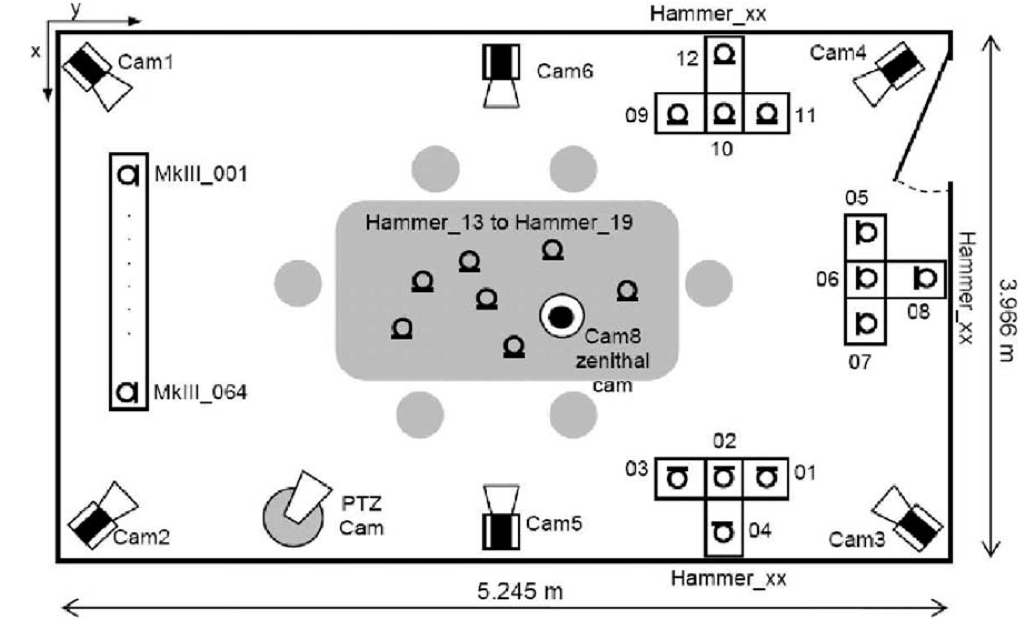
\includegraphics[scale=0.4]{figuras/3.TrabalhosCorrelatos/upc.png}
		\end{center}
		\caption{A configuração do ambiente inteligente UPC~\cite{salah}.}
		\label{upc}
	\end{figure}

Os sensores utilizados e as condições do ambiente inteligente UPC deste projeto são descritos pela Figura \ref{upc}. Os seguintes sensores foram utilizados:

	\begin{itemize}
		\item quatro câmeras nos cantos da sala (rotuladas como Cam1 a Cam4 na Figura \ref{upc});
		\item uma câmera \textit{zenithal fish-eye} no telhado (rotulada como Cam8 na Figura \ref{upc});
		\item uma câmera ativa apontada e com zoom para a porta de entrada para capturar as faces das pessoas que entram na sala (rotulada como PTZ na Figura \ref{upc});
		\item um \textit{array} de microfones NIST Mark III de 64 canais ;
		\item três \textit{clusters} de microfone de 4 canais no formato de T;
		\item oito microfones no teto;
	\end{itemize}


\begin{figure}[hbt]
		\begin{center}
			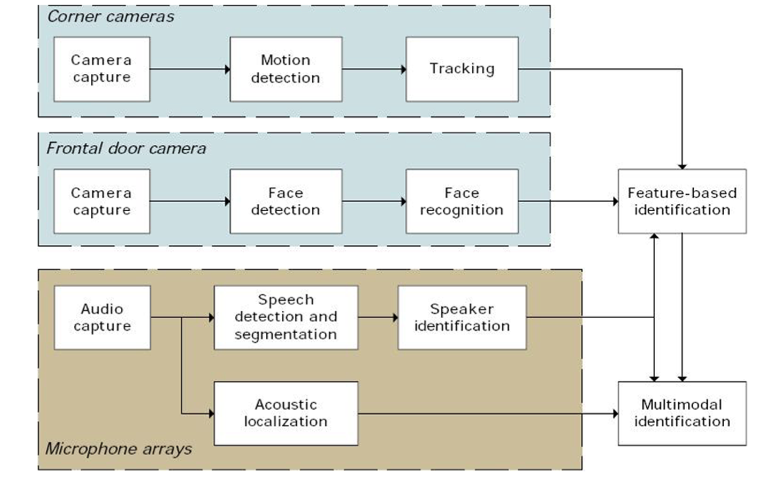
\includegraphics[scale=0.5]{figuras/3.TrabalhosCorrelatos/workflow.png}
		\end{center}
		\caption{\textit{Workflow} da informação na arquitetura do ambiente inteligente UPC~\cite{salah}.}
		\label{workflow}
	\end{figure}

As imagens coletadas pelas câmeras no sistema são utilizadas para detecção de movimento, rastreamento, detecção e reconhecimento facial e serão analisadas a seguir. Como mencionado, o sistema do projeto também promove localização dos usuários no ambiente, porém utiliza amostras de áudio como dados de entrada e por isso não será analisado.

\subsection{Detecção de movimento e Rastreamento}

A detecção de movimento utilizada tenta separar o ``primeiro plano'' do ``fundo'' para o seu funcionamento. O método que o projeto utiliza é baseado na detecção de objetos em movimento sob a suposição que imagens em uma cena sem objetos em movimento mostra regularidades, que podem ser modeladas utilizando métodos estáticos. O conjunto de treinamento é construído por sequências pequenas de gravações \textit{offline} feitas da sala vazia.

Para realizar o rastreamento foi utilizado a abordagem de um mapa de ocupação probabilística (\textit{probabilistic occupancy map} - POM)~\cite{pom} simplificado para ambientes internos, onde as trajetórias de movimentos são curtas e menos frequentes quando comparadas com trajetórias em ambientes externos. Somente as quatro câmeras nos cantos são utilizadas.

Nesta abordagem, o mapa de ocupação é utilizado para projetar a imagem de um esboço de uma pessoa (um retângulo simples) em cada visão das câmeras.  As sobreposições dos esboços e as detecções de movimento na imagem entre as várias câmeras indicam a presença de uma pessoa. A Figura~\ref{fig:pom} ilustra a distribuição da probabilidade de ocupação produzida pelo algoritmo. 

\begin{figure}[hbt]
		\begin{center}
			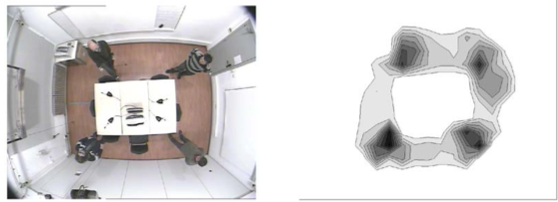
\includegraphics[scale=0.5]{figuras/3.TrabalhosCorrelatos/pom.png}
		\end{center}
		\caption{Mapa de ocupação probabilística. Adaptada de~\cite{salah}.}
		\label{fig:pom}
	\end{figure}

\subsection{Detecção e Reconhecimento Facial}

A detecção de movimento é feita utilizando o método \textit{Viola-Jones} já descrito anteriormente utilizando a biblioteca \textit{OpenCV}. 

Para realizar o reconhecimento facial utiliza uma técnica que aproveita a vantagem que o ambiente é constantemente monitorado e combina a informação de várias imagens para realizar o reconhecimento. As imagens das faces são fornecidas pelo módulo de detecção.
Para cada sequência de imagens, as faces de um mesmo indivíduo são agrupadas. Então, para cada grupo, o sistema compara as imagens com a galeria de imagens~\cite{salah}. 

Uma abordagem baseada em PCA (\textit{Principal Component Analisys}) foi utilizado para comparação entre as imagens.

%%%%%%%%%%%%%%%%%%%%%%%%%%%%%%%%%%%%%%%%%%%%%%%%%%%%%%%%%%%%%%%%%%%%%%%%%%%%%%%%%%%%%%%%%%%%%%%%%%%%%%%%%%%%%%%%%%%%%%%%%%%%%%%%%%%%%%%%%%%%%%%%%%%%%%%%%%%%%%%%%%%%%%%%%%%%%%%%%%%%%%%%%%%%%%%%%%%%%%%%%%%%%%%%%%%%%%%%%%%%%%%%%%%%%%%%%%%%%%%%%%%%%%%%%%%%%%%%%%%%%%%%%%%%%%

\section{Captura de contexto dinâmico e \textit{Arrays} de vídeos distribuídos para \textit{SmartSpaces}}

Esse trabalho apresenta detalhes de um projeto de pesquisa de longo prazo, onde \textit{SmartSpaces} de uma gama de funcionalidades úteis são projetados, construídos e avaliados sistematicamente. Algumas das funcionalidades chave incluem: detecção de intrusos; rastreamento várias pessoas; pose do corpo e análise de postura; identificação de pessoas; modelagem do corpo humano; e análise do movimento~\cite{trivedi}.

O sistema proposto monitora o ambiente em baixa resolução de forma contínua, detectando somente a presença e localização das pessoas e suas dimensões. Formas de aquisição de imagens mais detalhadas são ativadas quando um evento ou atividade de potencial interesse é detectado. Esses eventos serão os focos de atenção do sistema~\cite{trivedi}.

O monitoramento de baixa resolução e de grande área do ambiente é alcançado graças a algumas câmeras de amplo ângulo de visão e estáticas. Com um pequeno número de câmeras PTZ (\textit{pan/tilt/zoom}) ativas, múltiplos focos de atenção podem ser mantidos de forma simultânea~\cite{trivedi}.

Foi desenvolvido uma arquitetura de sistema para o \textit{SmartSpace} chamada DIVA. Ela pode ser vista como uma rede inteligente e ativa de câmeras, onde várias câmeras ão controladas para prover uma ampla gama de funcionalidades~\cite{trivedi}.

	\begin{figure}[hbt]
		\begin{center}
			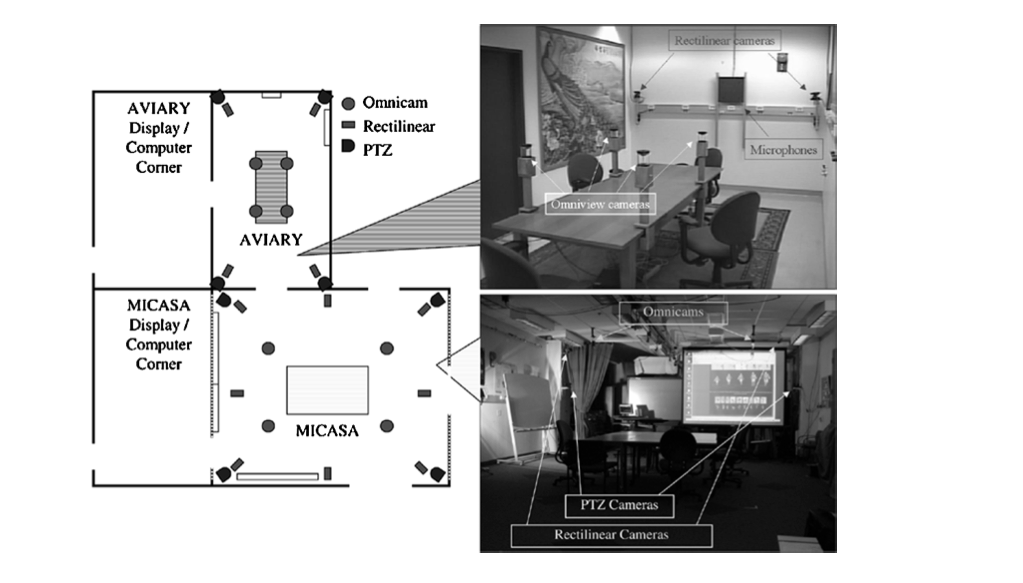
\includegraphics[scale=0.5]{figuras/3.TrabalhosCorrelatos/micasa_aviary.png}
		\end{center}
		\caption{Representação dos \textit{SmartSpaces} MICASA e AVIARY~\cite{trivedi}.}
		\label{micasa_aviary}
	\end{figure}

O projeto inclui dois \textit{SmartSpaces} separados, mas conectados. O primeiro é chamado de AVIARY foi projetado para ser uma pequena sala de conferências. O segundo chamado de MICASA foi projetado para ser uma pequena sala de aula. A Figura \ref{micasa_aviary} mostra fotos dos dois \textit{SmartSpaces} e como estão conectados, além da disposição dos sensores utilizados.

Os sensores na sala AVIARY incluem~\cite{trivedi}:

	\begin{itemize}
		\item uma rede de quatro câmeras omnidirecionais;
		\item quatro câmeras PTZ;
		\item quatro câmeras retilíneas estáticas;
		\item dois \textit{arrays} de microfones com quatro microfones cada;
	\end{itemize}

As quatro câmeras omnidirecionais (ODVSs) estão perto dos cantos de uma mesa de reunião, cobrindo o quarto inteiro de dentro para fora, como mostrado na Figura \ref{micasa_aviary}. As câmeras PTZ e retilíneas estão nos ``vértices'' da sala a $\displaysytle 1.4m$ acima do chão. Os dois \textit{arrays} de microfones foram instalados na parede e no teto~\cite{trivedi}.

Um computador é alocado para rastreamento, utilizando imagens das quatro câmeras omnidirecionais ou imagens das quatro câmeras retilíneas estáticas. Outro computador é utilizado para analisar os eventos de áudio e de vídeo. Um terceiro computador é utilizado para arquivar \textit{streams} de áudio e vídeo para posterior recuperação~\cite{trivedi}.

O \textit{SmartSpace} MICASA é duas vezes maior que o AVIARY. Os sensores utilizados nessa sala são~\cite{trivedi}:
	
	\begin{itemize}
		\item uma rede de quatro câmeras omnidirecionais;
		\item quatro câmeras PTZ;
		\item oito câmeras retilíneas státicas;
	\end{itemize}

As câmeras omnidirecionais são instaladas no teto, como mostrado na Figura \ref{micasa_aviary}. As câmeras PTZ e quatro câmeras retilíneas foram instaladas de maneira similar ao \textit{SmartSpace} AVIARY. As quatro câmeras retilíneas restantes foram instaladas nas paredes como mostrado como mostrado na Figura \ref{micasa_aviary}. As câmeras nos vértices possuem maior campo de visão para cobrir toda a sala e fazem parte do array de câmeras para rastreamento~\cite{trivedi}.

\subsection{Rastreamento, Detecção de faces e Reconhecimento facial}
 
Foi desenvolvido um sistema em tempo-real que utiliza a rede de câmeras omnidirecionais que é responsável pelo rastreamento, detecção das faces e reconhecimento facial. 

O rastreamento baseado na câmeras omnidirecionais é feito detectando a silhuetas das pessoas por meio da subtração do fundo com remoção de sombras.

O vídeo capturado é processado para detecção e reconhecimento de faces como mostrado na Figura \ref{facerec}. Para detecção de faces utiliza o método de segmentação de tom de pele. As imagens resultantes são classificadas para rejeitar as imagens sem faces. Então, o método \textit{Eigenface} é utilizado tanto para classificação da face quanto para reconhecimento. 

	\begin{figure}[hbt]
		\begin{center}
			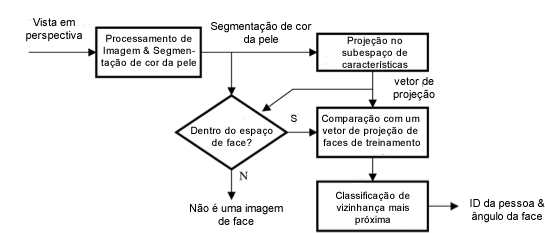
\includegraphics[scale=0.8]{figuras/3.TrabalhosCorrelatos/facerec.png}
		\end{center}
		\caption{Método de detecção e reconhecimento facial~\cite{trivedi}.}
		\label{facerec}
	\end{figure}














































